%authentication
\section{Authentication}
We have not implemented our own sign in option, since it would require us to handle the user's passwords and other personal information.
By using a social media sign in in our application as a way of identify the user, we move the security measures to the specific social media.
There are many different social media sign in options Google+, Facebook, Twitter etc., but the sign in we chosen to implement first is Google+. 
Google recommends using the Google+ sign in for Android applications\todo{kilde?}, since the developer is able to gather information about the user through their Google+ account. The other sign in option could later be implemented.

\subsection{Google+}
It makes sense to use Google+ sign in since it is highly recommended by Google to have a Google account when using an Android device, because the user would limit their experience with an Android device, if they do not have a Google account. 
The Google+ authentication is natively supported by Android and can be achieved seamlessly.  

In our implementation of the Google+ sign in we use a object called \\GoogleApiClient\citep{googleapiclient-docs}, which is provided by the Google Play services application. 
The object GoogleApiClient should be initialised and connected separately in every activity, so each activity has it own life cycle with the GoogleApiClient, \autoref{fig:googleclientlifecycle} shows the life cycle of a GoogleApiClient object in an activity.
\begin{figure}[H]
\centering
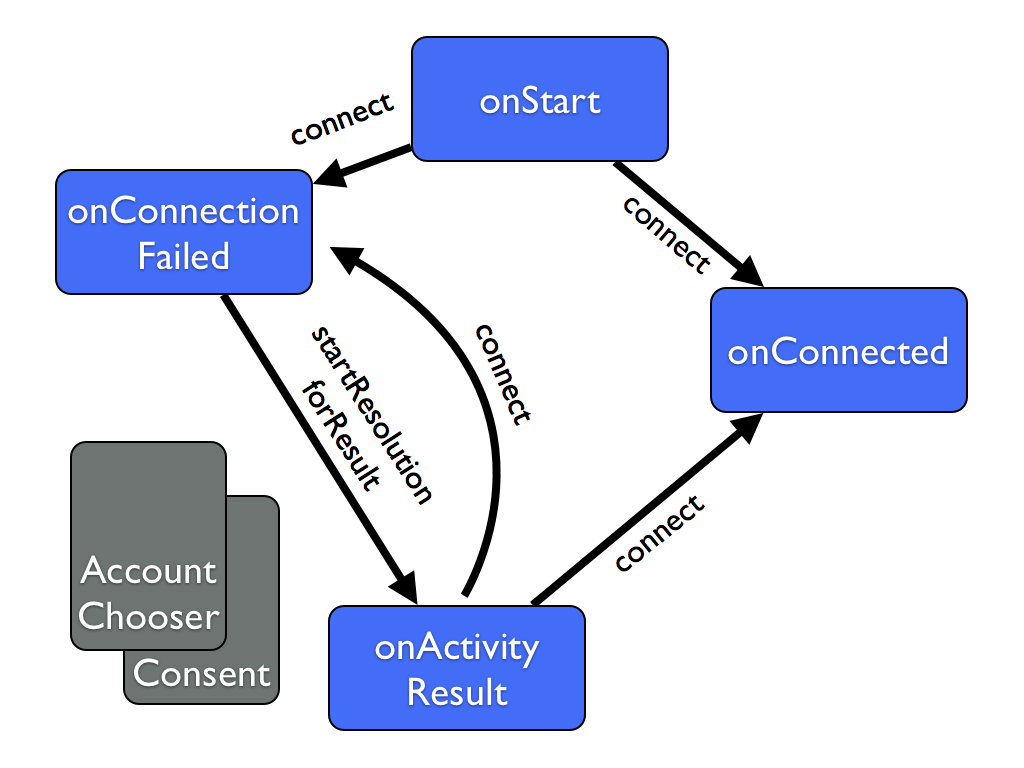
\includegraphics[width=0.8\linewidth]{img/googleclientflow.png}
\caption{The GoogleApiClient basic life cycle\cite{googleapiclient-lifecycle}}
\label{fig:googleclientlifecycle}
\end{figure}
The blue boxes represents methods in the activity, and the two grey boxes represents other activities. The method \textit{onStart()} is called upon the activity start up, and we immediately try to sign in. 
This can either succeed or fail, if it fails \textit{onConnectionFailed()} will be called, this will happen if the user has not yet consented with the Google+ sign in, the application now awaits for the user to press the sign in button. 
When the user presses the sign in button, the application opens an account chooser activity, if the user has multiple Google accounts. 
After selecting the account that the user want to use, a consent activity will show presenting the user with the Google+ information that the application should be allowed to access. 
When the user has granted the application access, the result of the consent activity is returned to \textit{onActivityResult()}, the user is signed in. 
If the user did not grant access to the application the routine starts all over. When the user is connected \textit{onConnected()} is called, this method simply updates the UI and downloads information from the user's Google+. 

When the user is signed in to our application we can get information of the user by using the GoogleApiClient.
In our application we only use the user's Google email(account name) and the user's real name(for comments on recipes). 
When we receives the user's email we hash it using a hashing technique called "SHA256", we do it because we can only use the uniqueness of the email, and it makes no sense storing the user's email in plain text both in the application and database. 
So we hash it and every time the user makes an action that requires the user to be signed in, we send the hashed email to the server together with the action. 
It might seem overrated that we send the hashed email every time and not just an user id, but the mobile device is not required to have Internet\todo{Internet or connection to the server?} to be able to sign in using Google+. The sign in can be achieved locally on the mobile device, we have kept the functionality of signing in without Internet by doing as mentioned before.

